\documentclass[12pt, a4paper, openany]{book}
\usepackage[utf8]{inputenc}
\usepackage{fullpage}
\usepackage{amsmath}
\usepackage{amssymb}
\usepackage{graphicx}
\usepackage{mathtools}
\usepackage[comma,authoryear]{natbib}
\usepackage{listings}
\usepackage{color}
\usepackage{wrapfig}

\definecolor{dkgreen}{rgb}{0,0.6,0}
\definecolor{gray}{rgb}{0.5,0.5,0.5}
\definecolor{mauve}{rgb}{0.58,0,0.82}

\lstset{frame=tb,
  language=R,
  aboveskip=3mm,
  belowskip=3mm,
  showstringspaces=false,
  columns=flexible,
  basicstyle={\small\ttfamily},
  numbers=none,
  numberstyle=\tiny\color{gray},
  keywordstyle=\color{blue},
  commentstyle=\color{dkgreen},
  stringstyle=\color{mauve},
  breaklines=true,
  breakatwhitespace=true,
  tabsize=3
}
\frenchspacing
\linespread{1.2}
\graphicspath{{./}}
\title{Modeling and Forecasting US Airline Flight Delays\\2020 TAMIDS Data Science Competition}
\author{Big Data Energy\\Johnathan Lo \& Isaac Ke\\Advisor: Dr. Huiyan Sang}
\date{April 8, 2020}

\newcommand{\R}{\mathbb{R}}
\newcommand{\Z}{\mathbb{Z}}
\newcommand{\Lagr}{\mathcal{L}}
\newcommand\tab[1][1cm]{\hspace*{#1}}

\begin{document}
\maketitle
\tableofcontents
\chapter{Introduction}
\tab Reliable transportation supports a strong economy by facilitating the rapid and timely exchange of goods and services and bolstering tourism revenue. In the United States in 2018, the transportation industry accounted for \$648 billion per year, which was 3.16\% of the GDP [cite]. Worldwide, the aviation industry contributes \$2.7 trillion (3.6\%) of the world's GDP. In fact, it is projected that global air transporation will support \$5.7 trillion of the global economy [cite]. A key metric for evaluating the efficiency of airline industry production is flight delay time. In 2018, flight delays led to an economic loss of 31.2 billion dollars[cite]. For individual companies, delays can influence consumer choice, and for the industry itself, unmitigated delays can impel consumers to switch to substitute goods, such as automotive or rail-based transport. \\
\tab Therefore, a major goal of this project is to analyze flight delays and diagnose areas for improvement. We intend to create models using the provided dataset as well as publicly available data that can accurately predict future delays. In doing so, we can hopefully uncover significant and controllable covariates that can help guide airline companies to reduce flight delays. 
\chapter{Executive Summary}
	\section{Problem and Approach}
\tab Ever since the first commercial airline flight was flown in 1914, the air transportation industry has played an integral part in both boosting the global economy as well as connecting people from all over the ever-interconnected world. On occasion, flights can be delayed from their scheduled times, and this results in lost revenue and irritated customers. The goal of our analysis was to not only model flight delays but also create predictive models to forecast future late arrivals, specifically for the third quarter of 2019. We dove into this project by first gathering and tidying up our data, performing exploratory data analysis, then fitting and assessing unique predictive models. By gathering substantive knowledge about airlines we then interpreted and applied our results with the intent to provide airlines with detailed areas to focus on to mitigate delays. Given a limit on resources, our goal was to uncover trends and pinpoint factors that can be controlled to help alleviate untimely arrivals. Intentional and thorough analysis was out driving force since quantitative evidence is what best drives changes in businesses.
	\section{Data Preprocessing}
\tab In addition to the datasets provided to us, we worked to gather historical weather information for all 11 million flights at both the origin and destination airport by fetching pertinent data from the NCDC (National Climate Data Center) API. After all data was gathered, we ensured our data was “tidy” by combining all flight, weather, airfare, route, airport, and geographical data into one data frame with each observation as a row and column as a covariate. Moreover, we changed appropriate covariates to categorical variables, replaced all missing values with reasonable entries, and experimented with transformations of variables. For subsequent models, data were further reorganized to fit the nature of the problem. For example, for one of our models we formatted the data to resemble longitudinal panel data. 
	\section{Exploratory Analysis}
\tab During the exploratory phase, we produced various plots and summary statistics to learn about the distribution and nature of flight delays. By using numerous packages in R along with connection to the Google maps API, we were able to produce numerous revealing plots. Among these, we were able to assess the geographic, temporal, carrier, and weather-based patterns of flight delays, to name a few. Through the construction of conditional density estimates and other tests, the main takeaway from our exploration was that flight delays are not a purely random event and that they behave very predictably across a myriad of factors. This motivated us to pursue the models that we did. 
	\section{Model Creation \& Assessment}
\tab Using the empirical distributions found during our exploratory analysis, we create a parametric distribution for the marginal values of the response. A parametric distribution is useful here because it provides interpretability and allows regression and Bayesian methods to be used on the parameters. A key difficulty here was the skewness of the distribution, which we could not correct through Box-Cox transformation. Attempts to fit other well-known distributions also failed. Ultimately, we decided on a mixture distribution, $Y = UV+(1-U)T$ where $U\sim Ber(p)$, $V\sim exp(\lambda)$, and $T\sim N(\mu, \sigma^2)$. The central idea behind this distribution is that most delays are ordinary, while some delays are the result of rare circumstances; the dichotomy between these two types of delays is determined by the parameter $p$, which is in turn determined by some hidden combination of variables. While using a parametric distribution is limiting in many ways, it also has descriptive utility in interpreting results. Using QQ plots and conditional density estimation, we were able to validate this parametric distribution for the majority of factor levels. Importantly, the conditional densities have the same approximate type of distribution. This distribution is henceforth referred to as the Lo-Ke distribution.
\tab Having the form of the conditional distributions allows us to construct linear models using OLS. Non-normality of the errors prohibits conventional inference procedures; however, the assumptions for Gauss-Markov are not violated and thus the OLS estimates still produce the best linear unbiased estimates. Moreover, the large sample size allows us to conduct inference using the standard formulae over most of the domain. Finally, to allow for prediction, we incorporate the Lo-Ke distribution to describe the errors. Since the distribution is not location-scale parameterized, we instead approximate by keeping other parameters constant while varying $p$. \\
\tab As we found that modeling the binary variable of whether or not a delay would occur was beneficial, we trained a logistic regression model. By splitting our data into training and testing sets, we regressed on the now-binary arrival delay response on a variety of other pre-departure factors such as weather conditions. We when generated a Receiver Operating Characteristics curve as well as a confusion matrix to further optimize our model and maximize its accuracy. \\
\tab Our linear regression showed some patterns in the residuals that we thought might be the result of autocorrelation. To deal with these effects, we fitted a dynamic linear model by creating a bootstrap time series and fitting a multi-season ARIMA. We then fitted a linear model using OLS to the residuals. 
	\section{Applications and Conclusions}
\tab The models we chose showed significant effects on arrival time for several different predictors. The most significant and predictable of these are seasonal effects by quarter and by time of day. Flights during the 2nd and 3rd quarters were both significantly and substantially later than flights during the 1st and 4th. Time of day shows a clear effect with lower delays in the early morning, and delays peaking for flights departing around 5 pm. Day-of-week effects were also observed, with Thursday and Friday having the greatest delays. However, these differences, though significant, were not substantial. Different carriers also showed significant differences in mean arrival time. While most large airlines performed around the middle of the pack, several, notably Delta and Alaska Airlines, performed much better than expected, given their routes and revenue. Among quantitative delays, latitude, longitude, and precipitation showed usefulness as predictors.\\
\tab Overall, model constructing was challenging with this dataset, not only because of its size, but because of the inherent difficulty in capturing all the possible sources of variation in flight delays. Every flight is made possible by the coalescence of hundreds, if not thousands of disparate factors; conversely, delays can result from a single anomaly among those. We can only conclude that airline statisticians have done an adequate job of finding and correcting most obvious sources of flight delays, as most of the factors that we uncovered are out of the control of airlines themselves. 
	
\chapter{Motivation, Data Description, and Software}
	\section{Motivation}
	\tab As stated in the introduction, flight delays can have a wide-ranging effect on the economy. Most airline companies have already done everything in their power to mitigate and reduce delays. We are interested in finding whether delays can be further alleviated, and whether those variables can be controlled by airline companies. To the extent that some delays are unavoidable or difficult to predict, we are also interested in devising methods to minimize the impact of those delays, whether by reducing the number of passengers affected, offering alternate routes to affected passengers, or discounting tickets. Overall, for the benefit of airline companies, consumers, and society-at-large, we should minimize flight delays, or the impact thereof. 
	\section{Data Collection}
	\tab Our data was provided as .csv files by the competition organizers. The primary dataset was composed of roughly 11 million observations of 50 variables. Each observation was a distinct flight that occurred between 1/1/2018 and 6/30/2019, and the 50 covariates included origin, destination, quarter, arrival delay, departure delay, distance, and many more variables pertaining to each flight. Auxiliary datasets included information on flight routes, airports, and market share. \\
	\tab In addition to these data, we also sought out additional data to enhance our analysis. We obtained geographic coordinates for each airport from \textit{openflights.org} [cite] and historical weather data from the NOAA databases through the NCDC API [cite]. The geographic coordinates are given in decimal format, and our weather data describes meteorological events near the origin and destination of each flight. Importantly, data \textit{along} the flight path was not obtained, due to time constraints and complexity. Also, a key was obtained to connect to the Google Maps API through their Google Cloud Platform. Various plots were created using this connection. A full list of covariates along with brief descriptions can be found in \underline{Supplementary Table 1}. 
	\section{Software}
	\tab All analyses were performed in R v3.6.3 using the RStudio IDE [cite]. Packages used include, but are not limited to, \textit{ggplot2}, \textit{ggmap}, \textit{dplyr}, \textit{caret}, \textit{rnoaa}, and \textit{tseries}. Individual datasets were loaded as \textit{data.frame} objects and combined using \textit{merge} along with various \textit{dplyr} commands . In addition, Microsoft Power BI was utilized in order to tidy the data and perform computationally-intensive data rearranging. The final dataset can be found as a .csv file in \underline{Supplementary Data 1}.
	
\chapter{Exploratory Data Analysis}

	\section{Data Wrangling}
	
	\tab Our dataset was drawn from four different main sources - flight delays and airfare data, geographic coordinates from \textit{openflights.org}, and weather data from NOAA. Flight delays and geographic coordinates were combined by merging on both common origin and destination names. The resulting data frame was then combined with fare/market data by common routes, year, and quarter. Adding weather data was more challenging in that the observations related information collected by weather stations, and not the airports themselves. Thus, weather station coordinates were cross referenced with airport coordinates to find the closest active weather station to each airport. Due to this constraint, 10 airports, corresponding to 99,980 observations (a negligable amount given the overall size of our data), were dropped due to the lack of NOAA weather stations nearby. Weather data was then merged with the rest of the data on common dates and airports, with separate variables for weather at origin and weather at destination. The final dataset containing all four sets of information is what will be referenced in this paper hereafter. Small tweaks to these data were made on a model-to-model basis, depending on the type of unique problem selected-whether it be classification or regression, for example. \\
	
	\tab The data contained a number of variables with numerical values but that could be interpreted either as quantitative or categorical variables. Using substantive knowledge, a number of numeric variables were converted to factors, including day of week, month, quarter, and route number. Additionally, our data contained many missing values. Where applicable, for categorical variables, these values were replaced by adding an additional factor level \textit{Unk}. For quantitative variables, missing values were replaced with either 0, or observations were removed, based on substantive knowledge of the variable characteristics. Finally, we discovered that the flight delay dataset somewhat bewilderingly assigned canceled flights a delay time of 0. Canceled flights were removed from the dataset and analyzed separately. Thoughout this report, we further to flight delays as specifically arrival delays as opposed to departure delays. In all, the final dataset consisted of 10,614,150 observations of 100 variables. 
	
	\section{Distribution of Flight Delays}
	
	\tab The dataset provided information on flights from 17 different carriers along 6,684 unique routes being flown between a combination of 362 airports in the United States (including Alaska and Hawaii and a couple airports in US territories such as Guam). 3,814,366 out of the 10,915,495 flights (~35\%) had some form of arrival delay. A histogram of all arrival delays is shown in \underline{Fig 4.1}. We observe that most "early" flights are not incredibly early compared to the frequency at which late flights can become "significantly" delayed, say more than 30 minutes. Clearly, the data is strongly right-skewed. To correct the skewness (to meet assumptions for our analysis), a cube-root transformation was performed, but subsequent Shapiro-Wilk tests provided strong evidence against normality for this transformation, so we turned to other methods, as will be discussed in chapter 5. To heuristically assess dependence between covariates and late arrivals, we examined various conditional distributions, as follows.\\
	\begin{wrapfigure}{l}{0.45\textwidth}
	\centering
	 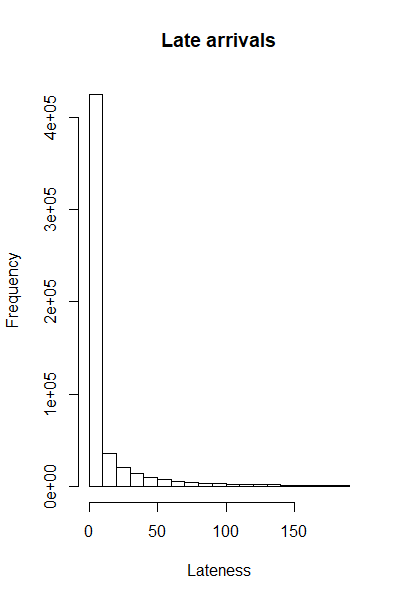
\includegraphics[width = .45 \textwidth]{../figures/LateArrivalsHistogram}
	 \caption{Fig 1 - Histogram of arrival time for all observations in the dataset}
	 \end{wrapfigure}
	 
		\subsection{Geographic Distribution of Flight Delays}
		
			\tab In \underline{Fig 4.21}, the routes that have various average intervals of delay time are shown. Note straight lines are drawn for simplicity; the actual flight most likely flew a non-linear path toward the destination. Also, early arrivals are given a delay time of 0 in the computation of the mean. We observe many things. Almost all routes have an average delay that is positive. This spotlights the nature of this project: to focus on remedying delays to improve customer satisfaction and increase airline revenue. For the routes with a mean delay between 30 and 45 minutes, most of the delays are clustered on the eastern US with most of the routes either beginning or ending in the San Francisco, New York, or southern Florida regions. For more severe delays of 45+ minutes, these routes encompass more cross-country flights. Furthermore, it can be seen that an airport in the northeast, most likely JFK in New York, is involved in a lot of severe flight delays. Next, in \underline{Fig 4.22}, the average delays at certain airports is depicted. We see further evidence that the more problematic delays are centered in bigger cities, particularly those on the east and west coast. \underline{Fig 4.23} illustrates the relationship between the popularity of an airport and the amount of delays. As expected, airports that crank out more flights have a higher average delay time. This raises the question: Does more flights simply give airports a higher probability of having delays (by random chance), or does an increase in flights also bring in other factors that \textit{cause} an increase in flight delays. In more broad terms, what factors correlate with delays, and which ones can be controlled by the airlines?\\
			\begin{wrapfigure}{r}{0.45\textwidth}
			\centering
	 		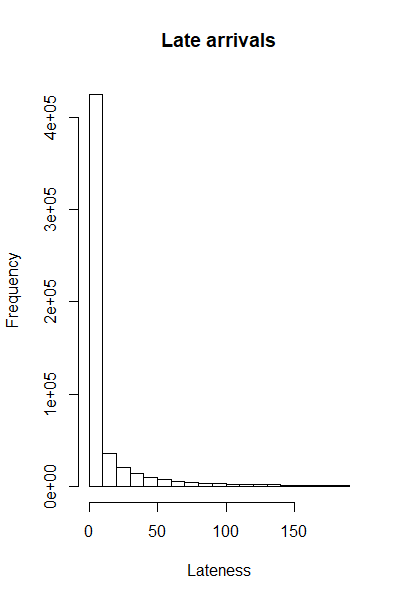
\includegraphics[width = .45 \textwidth]{../figures/LateArrivalsHistogram}
	 		\caption{Fig 2 - Figures showing the geographic distribution of flight delays by delay length and airport usage}
	 		\end{wrapfigure}
	 		
		\subsection{Temporal Distribution of Flight Delays}
		
			\tab \underline{Fig 4.31}, \underline{Fig 4.32}, \underline{Fig 4.33}, and \underline{Fig 4.34} display the distribution of flight delays for quarter, month, day of the week, and time of day, respectively. Note that because our data contained a year and a half’s worth of observations, the frequency of delays for quarter 1 and 2 are higher than other time periods that were not recorded twice. The histograms appear roughly symmetric with a slight right-skew. Specifically, early arrivals appear to follow a normal distribution while it transitions to an exponential distribution once delays become positive. We will explore this specific observation in the first section of our next chapter. Regardless, the general form of the distribution across these time factors does not change significantly. To further investigate the role of temporal factors in flight delays, we produced a number of coplots, which show several interesting seasonal patterns. \\
			\begin{wrapfigure}{l}{0.45\textwidth}
			\centering
	 		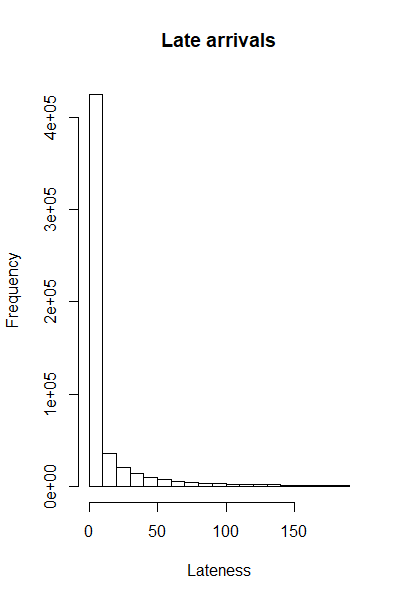
\includegraphics[width = .45 \textwidth]{../figures/LateArrivalsHistogram}
	 		\caption{Fig 3 - Histograms of ARR DELAY by time of day, day of week, month, and quarter}
	 		\end{wrapfigure}
	 		
		\subsection{Weather-based Distribution of Flight Delays}
		
			\tab This most obvious factor that most likely affects flight delays is the weather. Therefore, we analyzed the conditional distributions of flight delays given average temperature, precipitation, and the presence of various rare weather events. These are described in \underline{Fig 4.41}, \underline{Fig 4.42}, and \underline{Fig 4.43}, respectively. In the scatterplot depicting rain, we see a lack of evidence that more extreme temperatures correlate with increased delays. This would be evident if the scatterplot showed a parabolic pattern, which is not seen. Surprisingly, we see the same idea in the scatterplot of precipitation. Contrary to intuition, as the amount of precipitation increase, there is no visual subsequent increase in the delay time. Lastly, \underline{Fig 4.43} demonstrates that some dangerous weather events have a slightly bigger effect on delay times than others. For example, the distributions of “ice, sleet and hail” and “blowing or drifting snow” have more area in their right-tails. This is indicative of more occurrences where these events caused more significant delays. Besides these difference in tail-density, the overall shape remains very similar. \\
			\begin{figure}[h]
	 		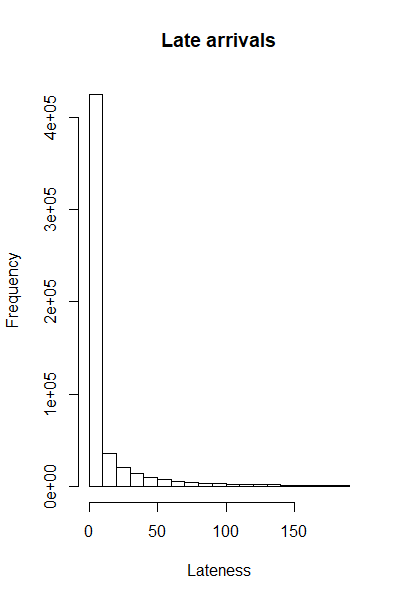
\includegraphics[width = .75 \textwidth]{../figures/LateArrivalsHistogram}
	 		\caption{Fig 4 - scatterplots of ARR DELAY by precipitation and temperature}
	 		\end{figure}
	 		\begin{figure}[h]
	 		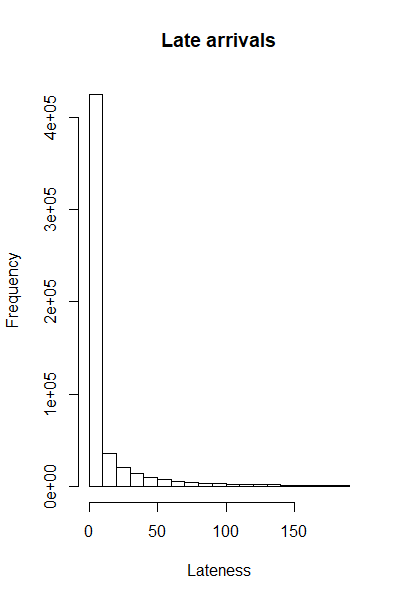
\includegraphics[width = .75 \textwidth]{../figures/LateArrivalsHistogram}
	 		\caption{Fig 5 - histograms of ARR DELAY for each unusual weather event}
	 		\end{figure}
		\subsection{Carrier-based Distribution of Flight Delays}
			
			\tab Next, looking at delays by carrier would provide us with insight as to whether some carriers are better at mitigating delays. \underline{Fig 4.5} shows us that the distribution across carriers stays roughly the same. Apart from the differences in frequencies (with some airlines being more popular or providing more flight routes), the shape of the distribution is basically homogenous, especially when compared to the other conditional distributions of other factors. This means that delays across carriers \textit{behave} in the same manner. To analyze if the average delay time (as opposed to distribution) differs across airlines, we conducted ANOVA (analysis of variance). Specifically, we used Tukey’s HSD to make multiple comparisons across each combination of carriers to see what carriers differed from one another. A plot of the resultant 95\% confidence intervals for the mean difference between airport delays is show in \underline{Fig 4.6}. We see that the majority of the intervals constructed do not fall within 0. Thus for those that didn’t, we conclude that they do indeed have a difference in mean arrival delays. All in all, we observe that the \textit{distribution} across carriers is similar, but the \textit{quantitative amount of delays} across carriers is different. \\
			\begin{figure}[h]
	 		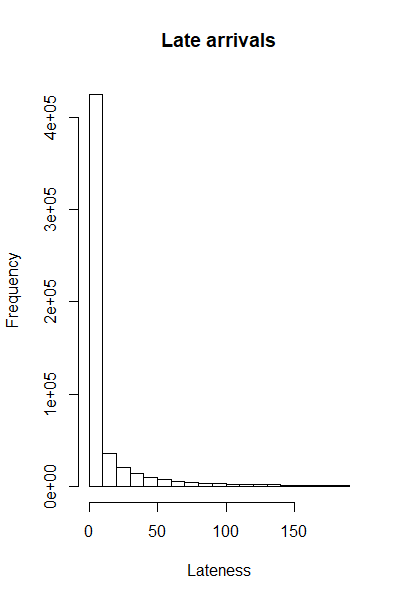
\includegraphics[width = 1 \textwidth]{../figures/LateArrivalsHistogram}
	 		\caption{Fig 6 - Histograms for the airlines}
	 		\end{figure}
	 		\begin{figure}[h]
	 		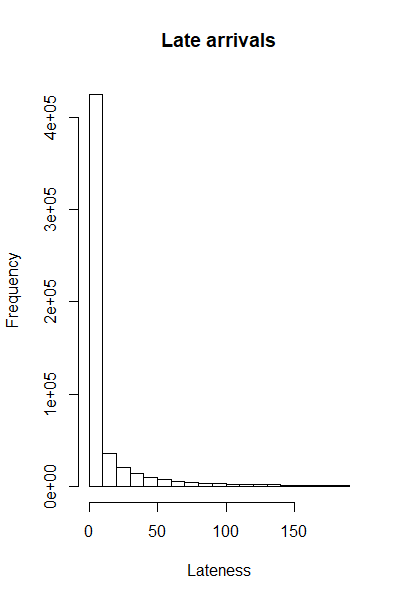
\includegraphics[width = 1 \textwidth]{../figures/LateArrivalsHistogram}
	 		\caption{Fig 7 - airline ANOVA}
	 		\end{figure}

		\subsection{Airport-based Distribution of Flight Delays}
			
			\tab \underline{Fig 4.7} displays the histograms of delays for some of the most popular airports. As has been the trend thus far, the distribution across the airports does not change much save for the changes in frequency. Thus, we can conclude the behavior and process of flight delays is pretty universal and can be modeled with an explicitly defined distribution, as we will dive into in the next chapter. \\ 
			\begin{figure}[h]
	 		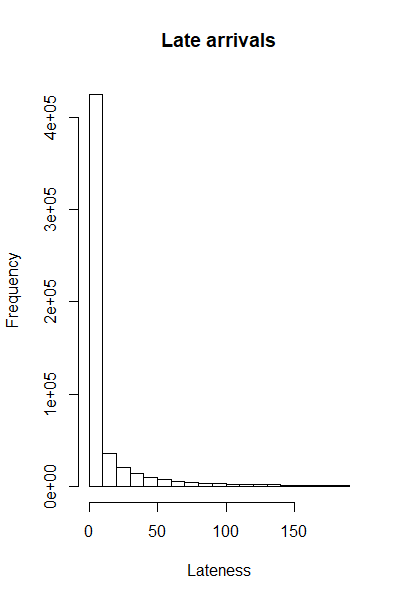
\includegraphics[width = 1 \textwidth]{../figures/LateArrivalsHistogram}
	 		\caption{Fig 8 - Airport histograms}
	 		\end{figure}

		\subsection{Making Up Lost Time En Route}
			\tab One last thing we wanted to explore was the ability for pilots to make up lost time as a result of a departure delay. We presumed that a longer flight, distance-wise, would allow for more opportunity for a flight delay to be alleviated. In the air, harnessing favorable air currents or taking shortcuts can remedy the lost time they left the ground with. Surely, in \underline{Fig 4.8}, we see that flights over a longer distance have, on average, less arrival delays. Similarly, the shorter the flight, the more severe the arrival delay is. These observations support our hypothesis stated above. Of course, correlation does not imply causation, so more substantive knowledge on how pilots navigate the flight route would provide more clarification on this. \\
			\begin{figure}[h]
	 		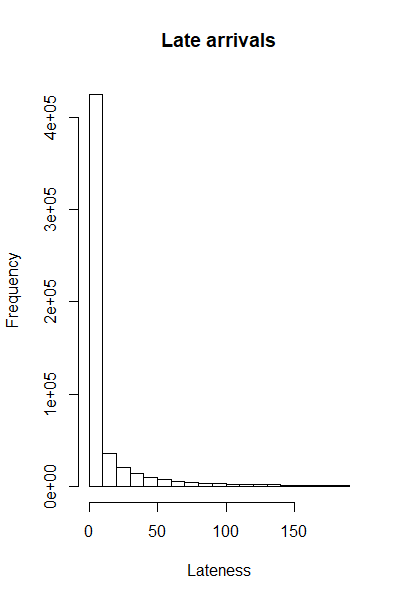
\includegraphics[width = 1 \textwidth]{../figures/LateArrivalsHistogram}
	 		\caption{Fig 4.8 - blah ablh}
	 		\end{figure}
	 		
\chapter{Model Formulation and Assessment}
	\section{Constructing a Parametric Distribution for \\Delays}
	 \tab We were interested in deducing the marginal distribution of arrival times from the data. Although it would have been relatively facile to estimate a valid empirical distribution, we decided that a parametric distribution would be more useful and intuitive. By establishing a set of parameters, further work could be directed towards estimating parameters under certain combinations of covariate values. With mostly categorical data, it then becomes feasible to estimate parameters for certain combinations of interesting variables. Parameterization also allows the density functions of the distribution to be readily expressed analytically.\\
	\tab As seen in \underline{Fig 1}, the marginal distribution is strongly right skewed, and thus our first plan of action was to attempt a transformation to correct the skewness. A number of transformations were considered. With negative values in the data, log or square root transformations could only be applied by first shifting the data to be strictly positive. One way to do this would be to simply add the smallest (most negative) number to each of our delay times; however, it was decided that this approach rendered our results somewhat uninterpretable. Consider, for example, a new observation where the flight arrived earlier (with a flight delay time more negative) than any other flight in the dataset. Such an observation would not be supported in a distribution of log-transformed values. We also briefly considered cube root transformation, but as seen in \underline{Fig 9}, it does not result in normality or resemblance to any familiar parametric distribution. In lieu of transforming the data, we considered several well-known skewed distributions, but none of them fit well or appeared sensible.\\
			\begin{wrapfigure}{l}{0.35\textwidth}
			\centering
	 		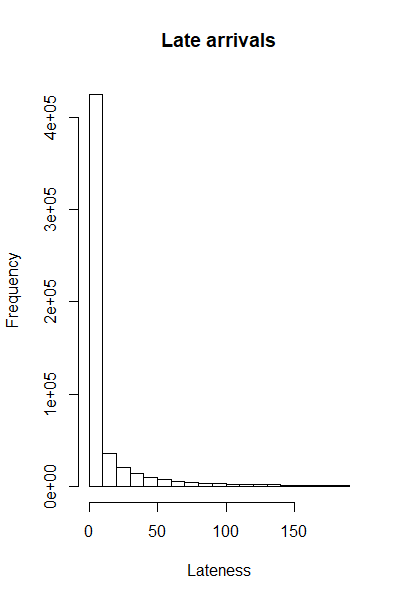
\includegraphics[width = .35 \textwidth]{../figures/LateArrivalsHistogram}
	 		\caption{Fig 9 - density plot of cube root transformation vs normal distribution with same mean and variance}
	 		\end{wrapfigure}
	\tab Thus, we instead looked to construct a mixture distribution. The primary issue that we had been confronted with this far was finding a distribution that appeared to have sensible parameterizations.  Our search was rooted in the premise that not all delays are created equal;  we suspected that the majority of delays are "run-of-the-mill" events that do not result from any extraordinary circumstances in particular, while a minority of delays have true, substantial causes. This is similar to the rationale for a zero-inflated Poisson in manufacturing processes, in that most machines are in good working order and do not produce any products with defects, but some machines with defects will produce defective products by a Poisson distribution. As such, we decided upon a mixture of the form \begin{center}$$Y = UV + (1-U)T$$\end{center} with $U\sim Ber(p)$, $V\sim exp(\lambda)$, and $T\sim  N(\mu,\sigma^2)$. In this model, $U$ describes whether or not a delay with "true, substantial causes" occurs, $T$ describes the distribution of arrival times when no extenuating circumstances occur, and $V$ describes arrival times under defined circumstances that result in lateness. The CDF of this distribution is given by 
	\begin{center}$$F_X(x) = \sum \alpha_i F_i(x) = p(1-e^{-\lambda x}) + (1-p)\left(\frac{1}{2}(1+ erf(\frac{x-\mu}{\sigma\sqrt{2}}))\right)$$\end{center}
	e.g. a simple mixture of two distributions. The pdf is given by \begin{center}
	$$f_X(x) = F_X'(x) = p(\lambda e^{-\lambda x} ) + (1-p)\left(\frac{1}{\sigma \sqrt{2\pi}} e^{-\frac{1}{2}(\frac{x-\mu}{\sigma})^2}\right)$$
	\end{center}
	Using MLE, we were able to generate estimates of the parameters for the marginal data, as shown in \underline{Fig 10}.\\
			\begin{wrapfigure}{l}{0.45\textwidth}
			\centering
	 		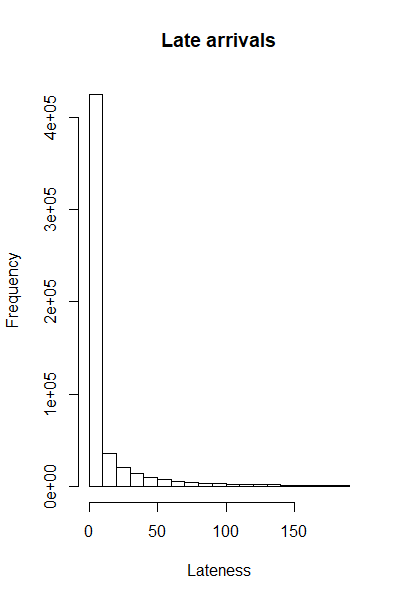
\includegraphics[width = .45 \textwidth]{../figures/LateArrivalsHistogram}
	 		\caption{Fig 10 - Histogram of samples from distribution given by MLE, and histogram of values from data (fig 9)}
	 		\end{wrapfigure}
	\tab To validate this distribution, a QQ plot was made of the observed arrival times against the mixture distribution under the parameter estimates from the MLE (\underline{Fig. 11}). From this plot, it can be observed that our mixture distribution is in fact able to describe the observed values of arrival time quite accurately. Note that the arrival times are given as discrete values (as minutes), hence the "jumps" from percentile to percentile. It is important to note here, however, that our distribution fails to describe data points in the extreme upper range of observations, p<.001. Some delays were quite extreme, with values in excess of 1000 minutes. To prevent such outliers from having outsize effect on our downstream analyses, we further pared the dataset here to include only data below the 99th percentile.  \\
			\begin{wrapfigure}{r}{0.45\textwidth}
			\centering
	 		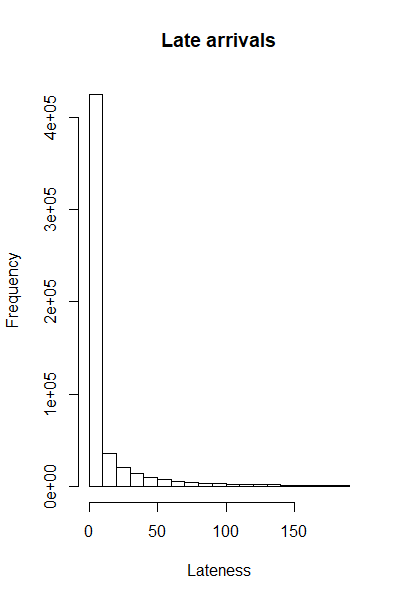
\includegraphics[width = .45 \textwidth]{../figures/LateArrivalsHistogram}
	 		\caption{Fig 11  - QQ plot of of data vs theoretical distribution}
	 		\end{wrapfigure}
	\tab Further, we see that conditional density estimation agrees with our theoretical parametric distribution. In \underline{Fig 12}, we show comparisons of the empirical conditional density vs densities given by our theoretical distribution with parameter estimates from MLE. Therefore, we suggest that our theoretical distribution can be used to describe arrival times across all combinations of factor levels. \\
			\begin{wrapfigure}{r}{0.45\textwidth}
			\centering
	 		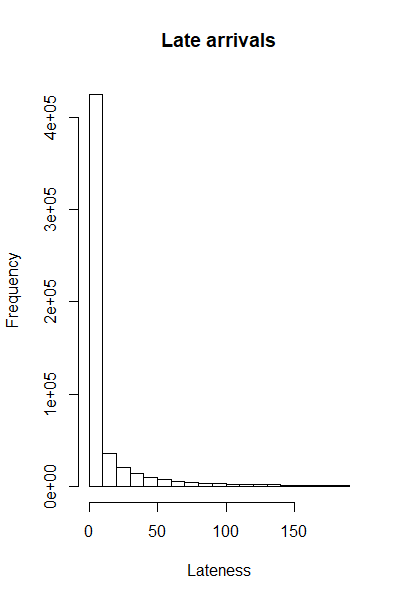
\includegraphics[width = .45 \textwidth]{../figures/LateArrivalsHistogram}
	 		\caption{Fig 12  - Comparison of several key conditional density estimates with our theoretical distribution}
	 		\end{wrapfigure}
	\section{Linear Model Using OLS}
	\tab Ideally, when constructing a linear model using OLS estimates, we want to satisfy four principal assumptions; namely, a linear relationship between predictors and response, independence of errors, homoscedasticity, and normality of the errors. However, having seen that the conditional distributions of the response are strongly \textit{non-normal}, and that there exists no simple transformation to restore normality, the fourth assumption appears to be violated. It is important now, to remember that, in fact, the Gauss-Markov theorem does \textit{not} require normality of the errors for the OLS estimates to be the best linear unbiased estimator, and that normally distributed errors are required only for conducting inference on the model via the t-distribution. For merely constructing a model equation and generating predictions that minimize mean squared error, normality of the errors is not strictly required. Further, inference on the model parameters can still be conducted through a variety of alternate methods. With heavy-tailed distributions of residuals, usually the more general M-estimation is used in place of OLS estimation, to provide robustness against non-normality when conducting hypothesis tests on model parameters. Alternatively, bootstrap can be used to generate the empirical error distribution. The size of our dataset, however, obviates the need for either of these procedures, since we can reasonably assume, by the Central Limit Theorem, that our estimates of the mean response, and therefore the coefficients of the model, are normally distributed. Therefore, the only inference that cannot be performed with the usual set of equations is prediction. \\
	\tab To conduct prediction, and construct prediction intervals, we use our theoretical distribution to distribute the errors. The predictions thus have the form: \begin{center}
	$$Y_{new}|X\sim X\beta + e$$
	with variance
	$$Var(Y_{new}|X) = X^TXVar(\beta) + Var(e)$$
	and
	$$E(Y_{new}|X) = E(X\beta)$$
	\end{center} 
	\tab The question then becomes how to select parameters for the theoretical distribution of our conditional responses. Particularly, how do the parameters relate to the mean and variance given above?  For errors that are normally distributed, or distributed via some member of the location-scale family of distributions, the parameters are precisely those given by the variance and expectation above. However, for our theoretiical distribution, solving for the correct parameter values becomes more challenging. Analytically, this requires either solving for the method of moments estimators or the MLE estimators. Both analytical solutions become complex rather quickly, for example, the moments of our theoretical distribution quickly get out of control:
	\begin{center}
	$$M_1 = \frac{p}{\lambda} +(1- p)\mu$$
	$$M_2 = p\left(\frac{2}{\lambda^2} - \frac{2\mu+1}{\lambda} - \mu^2 - \sigma^2\right) +\mu^2 +\sigma^2$$
	$$M_3 = \frac{6p}{\lambda^3} -(p+1)(\mu^3 + 3\mu\sigma^2) $$
	\end{center} 
	where we have used $M_i$ to denote moments rather than the usual $\mu_i$, to avoid confusion. To actually solve for the 4 parameters, we would also need a fourth moment. Likewise, for closed form MLE estimation, we would need to solve a system of 4 partial derivatives. While such a solution exists and is not as excruciatingly time consuming as it might appear, we can approximate a solution by conducting numerical MLE on a subset of data close to the given values of the predictors. 
	\section{Logistic Regression}
	\tab The majority of the models in data science can be put into three bins: regression, classification, and clustering. As we came to realize that our linear regression model was not useful enough, we turned to a classification method. In particular, we chose binary logistic regression to predict whether or not a flight would be delayed or not given certain pre-departure covariates. In retrospect, our motivation for pursuing logistic regression was two-fold. For one, we wanted to improve on the accuracy of our predictive model, so by moving away from regressing on a continuous variable, we shifted our focus to predicting a binary success or failure. Secondly, our conditional density estimates illustrate that given certain covariate levels, the shape of our distribution changes more than the mean (location) of our distribution. Thus, regressing on the parameter p from our Bernoulli random variable from our mixed distribution would help us explain these observed changes in our conditional density estimates. The marginal distribution of U in our model changes how thick-tailed our distributions become on either side of 0. \\
	\tab Using the \textit{glm()} function in R, we fit a generalized linear model using the logit function as the link function and the binomial distribution family as the probability distribution. A 5\% subset of our data frame was taken to shorten computation time. Even more, 80\% of our data was allotted for training and 20\% for testing. The summary of our fit model is show in \underline{Fig X.X}. Our covariates included various factors on the time as well as weather phenomena in the departure and arrival airport. We interpret our logistic regression output in two separate ways for numerical and categorical data. For numerical data, the specific factor level’s coefficient can be interpreted as the change in the log-odds of the “success” occurring – in our case a delay. Exponentiating these values gives you a more interpretable estimate. For example, from our model output, we can say that for every additional millimeter of snow, the odds of a delay occurring (versus not occurring) increases by a factor of $e^{0.1283}$ = 1.013. For categorial data, the interpretation is a little different. We illustrate by example. In our case, flying in April as opposed to January lowers one’s chances of having a flight delayed by a factor of $e^{-0.2646}$ = 0.767. Furthermore, we see that the majority of our coefficients are statistically significant as indicated by the asterisks next to each line. These significant predictors are thus being utilized in our model, as desired. \\
	\tab Since our logistic regression model outputted a \textit{probability} that a delay will occur, we needed to determine the optimal probability threshold to determine whether or not a delay will take place. We thus improved our model by plotting an ROC curve, or a “Receiver Operating Characteristics” curve (\underline{Fig X.X}. By maximizing the area under the curve, we are able to increase our accuracy. The y-axis gives the true positive rate while the x-axis gives 1 minus the true negative rate. Thus, by altering the probability threshold, we can then predict with better accuracy. Using this ROC curve and various functions, we found that the optimal probability threshold was 0.39. This means that any predictions that output the probability of a delay as being over 0.39, we say that a delay will occur. \\
	\tab Finally, after validating our model on the testing data, we generated a confusion matrix and other measures of performance as shown in \underline{Fig X.X}. Our accuracy was 67.62\% where out of our testing set of 92,667 observations, it correctly predicted 62,187 of them. Observe from the confusion matrix that we have significantly more false positives than false negatives. Thus, we interpret this as our model is more on the pessimistic side and is more likely to forecast a delay when in reality there is not one. \\

		
	\section{Time-Based Model: Dynamic Regression Model}
	\tab From our exploratory data analysis, we noted that several different categorical variables related to time showed significant effects on the mean arrival time. In particular, the scheduled time of a flight had a particularly noticeable effect on arrival delays over the course of a day. While our original linear model accounted for time-related effects by including aspects of the date and time as categorical variables, the assumptions of linear regression do not allow autocorrelation, which we believed could play a role in the true model of arrival times. For example, one could imagine that a flight that randomly arrives 10 minutes late could cause a subsequent flight to arrive $f(10)$ minutes late, where $f$ is some autocorrelation function. Thus, another possible model for arrival times would be 
	\begin{center}
	$$Y_t = X_t\beta + \eta_t$$
	\end{center}
	where $\eta_t$ represents the an error series following an ARIMA model. This model could then eliminate the aut We thought the data might have an underlying time series, so our approach here was to construct a time series and then perform regression on the residuals. 

	\tab Last but not least, we   From our data exploration, we see that for major covariates, we do not see a change in the general shape of the distribution itself, only small changes in the parameters. Based on this, we make the simplifying assumption that the conditional distribution is identical and independent across all combinations of factor levels, keeping in mind the limitations of this approach.  Furthermore, simplified model, use p instead of location parameter, show moments, describe strategy for producing conditional distributions of response based on 1st, 2nd, 3rd moments from data. Give equations. If the fixed effect model worked, then we would have fit that model and then fit a linear regression on the residuals to try to capture all effects. \\
	

\chapter{Forecasting Flight Delays for 2019 Q3}
	\section{Challenges}
	\tab Predicting flight delays can be challenging particularly because it is a subject that has already been investigated no doubt thoroughly by data scientists under the employ of the airline companies themselves. Many influential observations are the result of extreme values that happen rarely, while most observations are not so extreme. Black swan stuff, disparity in sample sizes, difficulty of incorporating models that can accurately predict rare, but highly impactful events (e.g. blizzards, tornadoes)
	\section{Using our Forecast Model}
	\tab Using our regression  model we predict  such and such requiring the following list of covariates. Based on time series data we have the following.
\chapter{Business Recommendations}
	\section{Differences Between Carriers}
	\tab Look at our ANOVA. Some of you guys suck.
	\section{Important Variables to Keep an Eye On}
	\tab The following variables are important to note. Some of these variables are not under control. Some variables are under control. What to do in each case. Some variables that may seem to be important but are not.
\chapter{Closing Thoughts}
	\section{Retrospect}
	\tab There are many possible approaches to this type of statistical problem, and given our limited statistical knowledge and computing power, it is difficult to intuit which would be best. In the end, many of our critical choices were subjective. We chose our response variable, the arrival delay time, based on our own preferences and experiences with air travel; we felt that the arrival delay would be the variable of interest for the majority of consumers, and the most economically impactful. Alternative choices like departure time or cancellation have their own justification. Additionally, the response could have been transformed in a number of different ways that could have made it more informative. For example, one might perhaps be interested in how long a delay might be only \textit{if} it occurs, in the delay time as a proportion of the original flight time, or some delay metric adjusted for the distance between origin and destination. Likewise, our choice of predictor variables was informed by our own background and objectives. For researchers with backgrounds in econometrics, it may be more interesting to study the dataset in the context of the economic environment of 2018-19. Finally, our choice of method for linking our predictors and our response was pivotal. Many other types of regression were briefly discussed, but most of them were too far outside our undergraduate expertise to earnestly consider.  \\
	\tab  Technology is the other key, and often underestimated, component of a successful statistical analysis. Being limited to our home computers for the majority of this exercise, we were unable to run algorithms requiring high computational loads. In such circumstances, it may have been wiser to familiarize ourselves with cloud computing services like Google Cloud before subjecting our own laptops to such heavy workloads. Many of our exploratory analyses took hours to days to run, only to find that them unsuccessful or underwhelming. However, overall, we feel that we leveraged the available technological resources to a satisfactory extent. 
	\section{Future work}
	\tab There are many potential analyses that can still be done on this dataset. One of the biggest roadblocks throughout the course of this exercise was our relative lack of computing power. With more computing assets, better machine learning algorithms, such as CNNs, MARS, and XGBoost could be applied. We believe that one of the strengths of our analysis was compiling a dataset that incorporated both the data given to us by the organizers, and large amounts of outside data. In fact, we still have copious amounts of outside data on airport characteristics, runway lengths, and airspace classes that would have been incorporated were it not for the physical restrictions imposed by our limited RAM. \\
	\tab The question of how best to ameliorate arrival delays remains an issue of core importance to the economy. Generations of statisticians have tackled this problem, and future generations will continue to. It is obvious that, the more delays are reduced, the more they can be extended, and hence, the more utility and convenience can be added to various modes of transportation. Thus, reducing delays is an important driver of technological progress in the transportation industry. Humans are too tolerant to ever eliminate delays entirely, and so the job of the statistician is simply to predict them as accurately as possible. 
\chapter{Appendix}
	\section{References}
	\section{Additional Figures, Tables, Code, and Data}
\pagebreak

\bibliographystyle{natdin}
\nocite{*}
\bibliography{sources}
\end{document}